% One figure containing six subfigures one for each positional state (three for rendezvous and three for docking) demonstrates the convergence of the chaser to the final state.
% Move the location of this figure based on placement aesthetics.
\begin{figure*}[htb]
  \begin{subfigure}[b]{0.33\textwidth}
    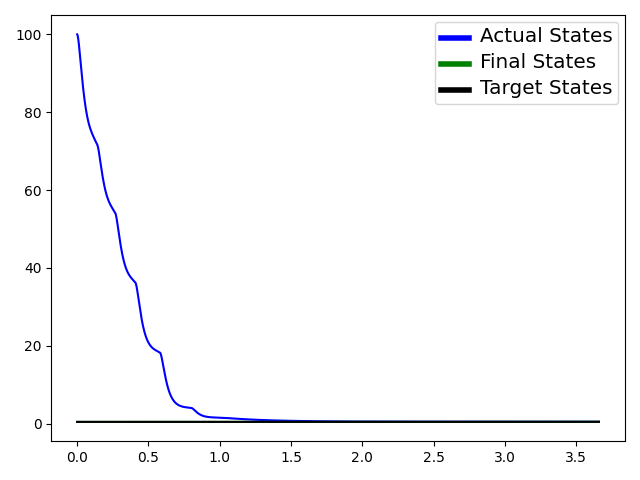
\includegraphics[width=\linewidth]{assets/complete_x_traj.png}
    \caption{Complete Trajectory in the X-axis}
    \label{fig:results_x_rnd}
  \end{subfigure}
  \hfill
  \begin{subfigure}[b]{0.33\textwidth}
    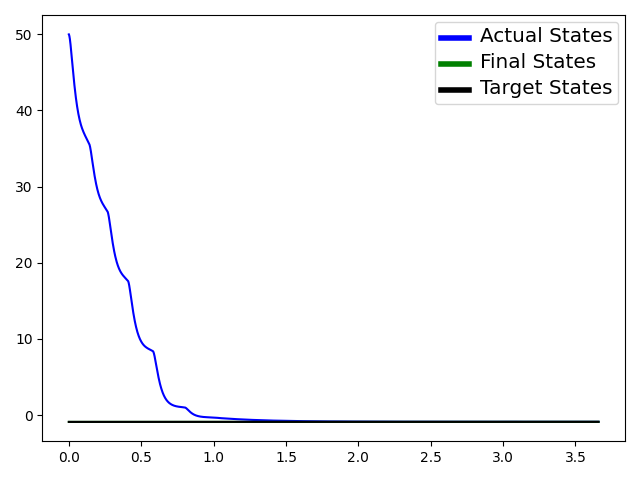
\includegraphics[width=\linewidth]{assets/complete_y_traj.png}
    \caption{Complete Trajectory in the Y-axis}
    \label{fig:results_y_rnd}
  \end{subfigure}
  \hfill
  \begin{subfigure}[b]{0.33\textwidth}
    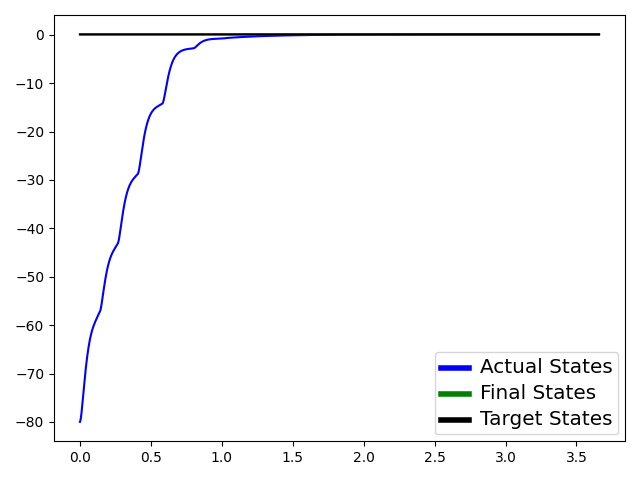
\includegraphics[width=\linewidth]{assets/complete_z_traj.png}
    \caption{Complete Trajectory in the Z-axis}
    \label{fig:results_z_rnd}
  \end{subfigure}
  \begin{subfigure}[b]{0.33\textwidth}
    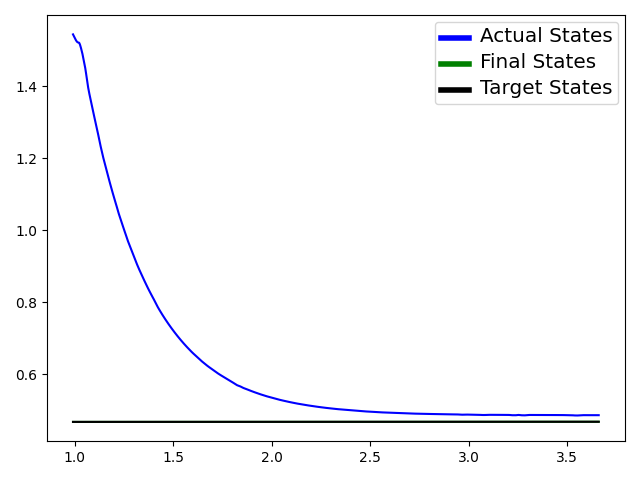
\includegraphics[width=\linewidth]{assets/docking_x_traj.png}
    \caption{Docking Trajectory in the X-axis}
    \label{fig:results_x_dock}
  \end{subfigure}
  \hfill
  \begin{subfigure}[b]{0.33\textwidth}
    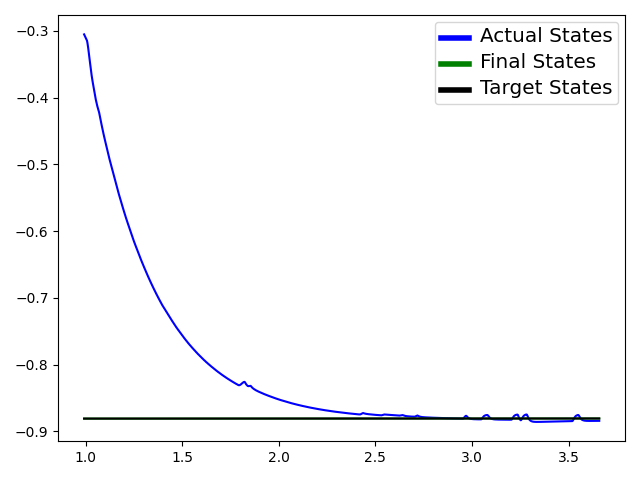
\includegraphics[width=\linewidth]{assets/docking_y_traj.png}
    \caption{Docking Trajectory in the Y-axis}
    \label{fig:results_y_dock}
  \end{subfigure}
  \hfill
  \begin{subfigure}[b]{0.33\textwidth}
    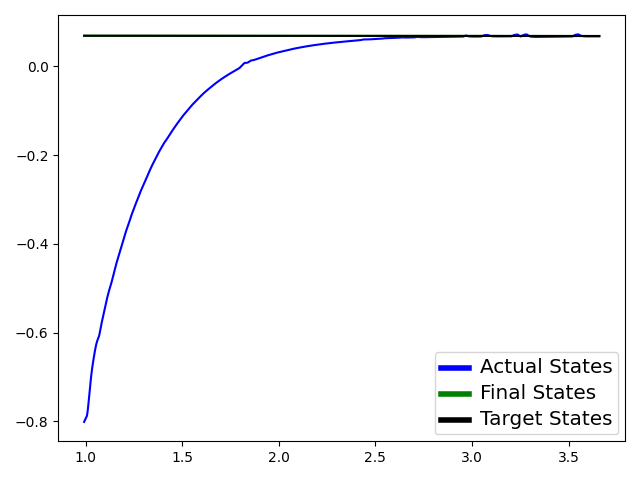
\includegraphics[width=\linewidth]{assets/docking_z_traj.png}
    \caption{Docking Trajectory in the Z-axis}
    \label{fig:results_z_dock}
  \end{subfigure}
  \caption{\textbf{Simulation of Rendezvous and Docking using Adaptive Dynamic Tube Model Predictive Control}: Subfigures \ref{fig:results_x_rnd}, 
 \ref{fig:results_y_rnd}, and \ref{fig:results_z_rnd} demonstrate the positional states of the chaser in the execution of the complete pipeline whereas subfigures \ref{fig:results_x_dock}, \ref{fig:results_y_dock}, and \ref{fig:results_z_dock} focuses on the positional states for the docking operation. Note that rendezvous ends and docking begins when the chaser is at less than 2.0 units away from the docking position.}
 \label{fig:results_pipeline}
\end{figure*}

\section{Target Deflection}
\label{sec:target-deflection}
Once the chaser has docked with the target at some position $\boldsymbol{d}$ with respect to the center of the target, any force $\boldsymbol{f}$ applied by the chaser thrusters translates to a torque $\boldsymbol{\tau}$ applied on the target as:
\begin{align}
    \boldsymbol{\tau} = \boldsymbol{d}\times\boldsymbol{f}
\end{align}
In the multi-agent scenario (with $N_C$ chasers), the net torque acting on the target can be written as:
\begin{align}
    \boldsymbol{\tau} = \sum_{i=1}^{N_C}\boldsymbol{d}_{i}\times\boldsymbol{f}_{i}
\end{align}
As a result, the dynamics of the target can be written using the Newton-Euler equations as follows:
\begin{align}
    \dot{\boldsymbol{\theta}}(t)&=\boldsymbol{\omega}(t)\\
    I\dot{\boldsymbol{\omega}}(t)&=-\boldsymbol{\omega}(t)\times I\boldsymbol{\omega}(t)+\sum_{i=1}^{N_C}\boldsymbol{d}_{i}\times\boldsymbol{f}_{i}
\label{eqn:newton-euler-target-detumbling}
\end{align}
This section focuses on the calculation of the optimal docking position and control input trajectory of the chaser(s) such that the final angular velocity of the target is zero while minimizing a cost function proportional to the net control input.
The interaction of multiple chasers with the target is more complicated than the single-agent case since one agent interacting with the object could change the environment for all other agents.
To simplify this issue, for the multi-agent scenario, we propose the simultaneous attachment of all chasers and the application of thrust so as to stop tumble only after all chasers have been attached to the target.\\
In this section, we retreat to the traditional form of representing, differentiating, and integrating variables with respect to time although the same operations may be performed using true anomaly as the independent variable.
% While the position of a chaser remains stationary after attachment, due to the tumbling nature of the target, the docking onto the target involves a time-varying final-position constraint which is considered in Eqn. \ref{}. For instance, if the target is cylindrical as demonstrated in Fig. \ref{} but revolves about an axis @@@ that does not pass through its center, the final position of each chaser is constrained to the following time-varying cylindrical surface:
% \begin{equation}
% \end{equation}
\subsection{Calculation of Docking Points and Force Application}
In order to calculate the docking points for each chaser $i\in[1,2,\ldots,N_C]$, we minimize the sum of the integral of forces applied by each chaser. This optimal control problem is governed by the Newton-Euler equations described above in Equation \ref{eqn:newton-euler-target-detumbling}. The moment of inertia and the initial angular velocity of the target is obtained from techniques such as polhode analysis as explained in Section \ref{sec:target-estimation}. Since the problem aims to stop the tumble of the target, the final angular velocity of the target is set to zero. Accounting for these constraints, the detumbling problem can be expressed as the following dynamic optimization problem:
\begin{alignat}{2}
    \min_{\boldsymbol{d}_{i},\boldsymbol{f}_{i}}\ &J\left(\boldsymbol{f}_{i}(t),\boldsymbol{d}_{i},\boldsymbol{\theta}_T(t), \boldsymbol{\omega}_T(t)\right)\\
    & =\int_{t_0}^{t_f} C\left(\boldsymbol{f}_{i}(t),\boldsymbol{d}_{i}, \boldsymbol{\theta}_T(t), \boldsymbol{\omega}_T(t)\right) dt\notag\\
    & =\int_{t_0}^{t_f}\sum_{i=1}^N||\boldsymbol{f}_{i}(t)||^2dt\notag
\end{alignat}
\begin{subequations}
\begin{alignat}{2}
    \textrm{s.t. } & \dot{\boldsymbol{\theta}}(t)=\boldsymbol{\omega}(t)\\
    & I\dot{\boldsymbol{\omega}}(t)=-\boldsymbol{\omega}(t)\times I\boldsymbol{\omega}(t)+\sum_{i=1}^{N_C}\boldsymbol{d}_{i}\times\boldsymbol{f}_{i}\\
    & \boldsymbol{\omega}(t_0)=\boldsymbol{\omega}_0,\quad\boldsymbol{\omega}(t_f)=0\\
    & \boldsymbol{f}_{i}\in{\mathbb{F}}_i\\
    & \boldsymbol{d}_C\in{\mathbb{G}}_T \label{eqn:geometrical-constraint}
\end{alignat}
\end{subequations}
Here, ${\mathbb{F}}_i$ represents the input bounds on chaser $i$ and ${\mathbb{G}}_T$ represents the geometrical constraint of the target on the docking point of the chaser. For example, if the target is a cylinder of radius $r_T$ and length $2l_T$ centered at the origin (assuming docking on the curved surface), the geometrical constraint in Equation \ref{eqn:geometrical-constraint} can be expanded as:
\begin{align}
    {\mathbb{G}}_T&={\mathbb{G}}_{T1}\cap{\mathbb{G}}_{T2}\\
    {\mathbb{G}}_{T1}&=\{\boldsymbol{d}_C:\boldsymbol{d}_{C,x}^2+\boldsymbol{d}_{C,y}^2=r_T^2\}\\
    {\mathbb{G}}_{T2}&=\{\boldsymbol{d}_C:|\boldsymbol{d}_{C,z}|<l_T\}
\end{align}
For the problem of calculating docking points, we ignore the rotation of the target. Instead, this rotation is considered in the formulation of the final state constraint for the docking trajectory problem as shown in Section \ref{sec:time-varying-final-state-constraint}.
\subsection{Discretization of Docking Points}
Due to the likelihood that specific points on the target (such as existing docking ports) will support docking better than others, we propose extending the above problem such that the docking position $\boldsymbol{d}_{i}$ lies in a discrete set of positions on the target.
As a result, the continuous geometrical constraint on the position of the chaser given in Equation \ref{eqn:geometrical-constraint} turns into the following discretized constraint:
\begin{align}
    \boldsymbol{d}_{i}&\in\begin{bmatrix}
        \boldsymbol{d}_{T_1}&\boldsymbol{d}_{T_2}&\ldots&\boldsymbol{d}_{T_j}&\ldots&\boldsymbol{d}_{T_M}
    \end{bmatrix}
\end{align}
hence converting the problem to a mixed-integer nonlinear optimal control.
To avoid the complexity involved in solving mixed-integer problems, we define the final position $\boldsymbol{d}_{i}$ for each chaser $i\in[1,2,\ldots,N]$ as follows:
\begin{align}
    o_{i,j}^2-o_{i,j}&=0\ \forall\ j\in[1, 2, \ldots, M]\\
    \sum_{j=1}^Mo_{i,j}&=1\\
    \boldsymbol{d}_{i}&=\sum_{j=1}^Mo_{i,j}\boldsymbol{d}_{T_j},
\end{align}
following which we convert equalities to approximate inequalities for solver convergence:
\begin{align}
    \cdot&=0\iff\lim_{\epsilon\rightarrow0}|\cdot|<\epsilon
\end{align}